\section{Sprache zur Klassendefinition}
    \subsection{Sprachkonzepte}
        \begin{figure}
            \centering
            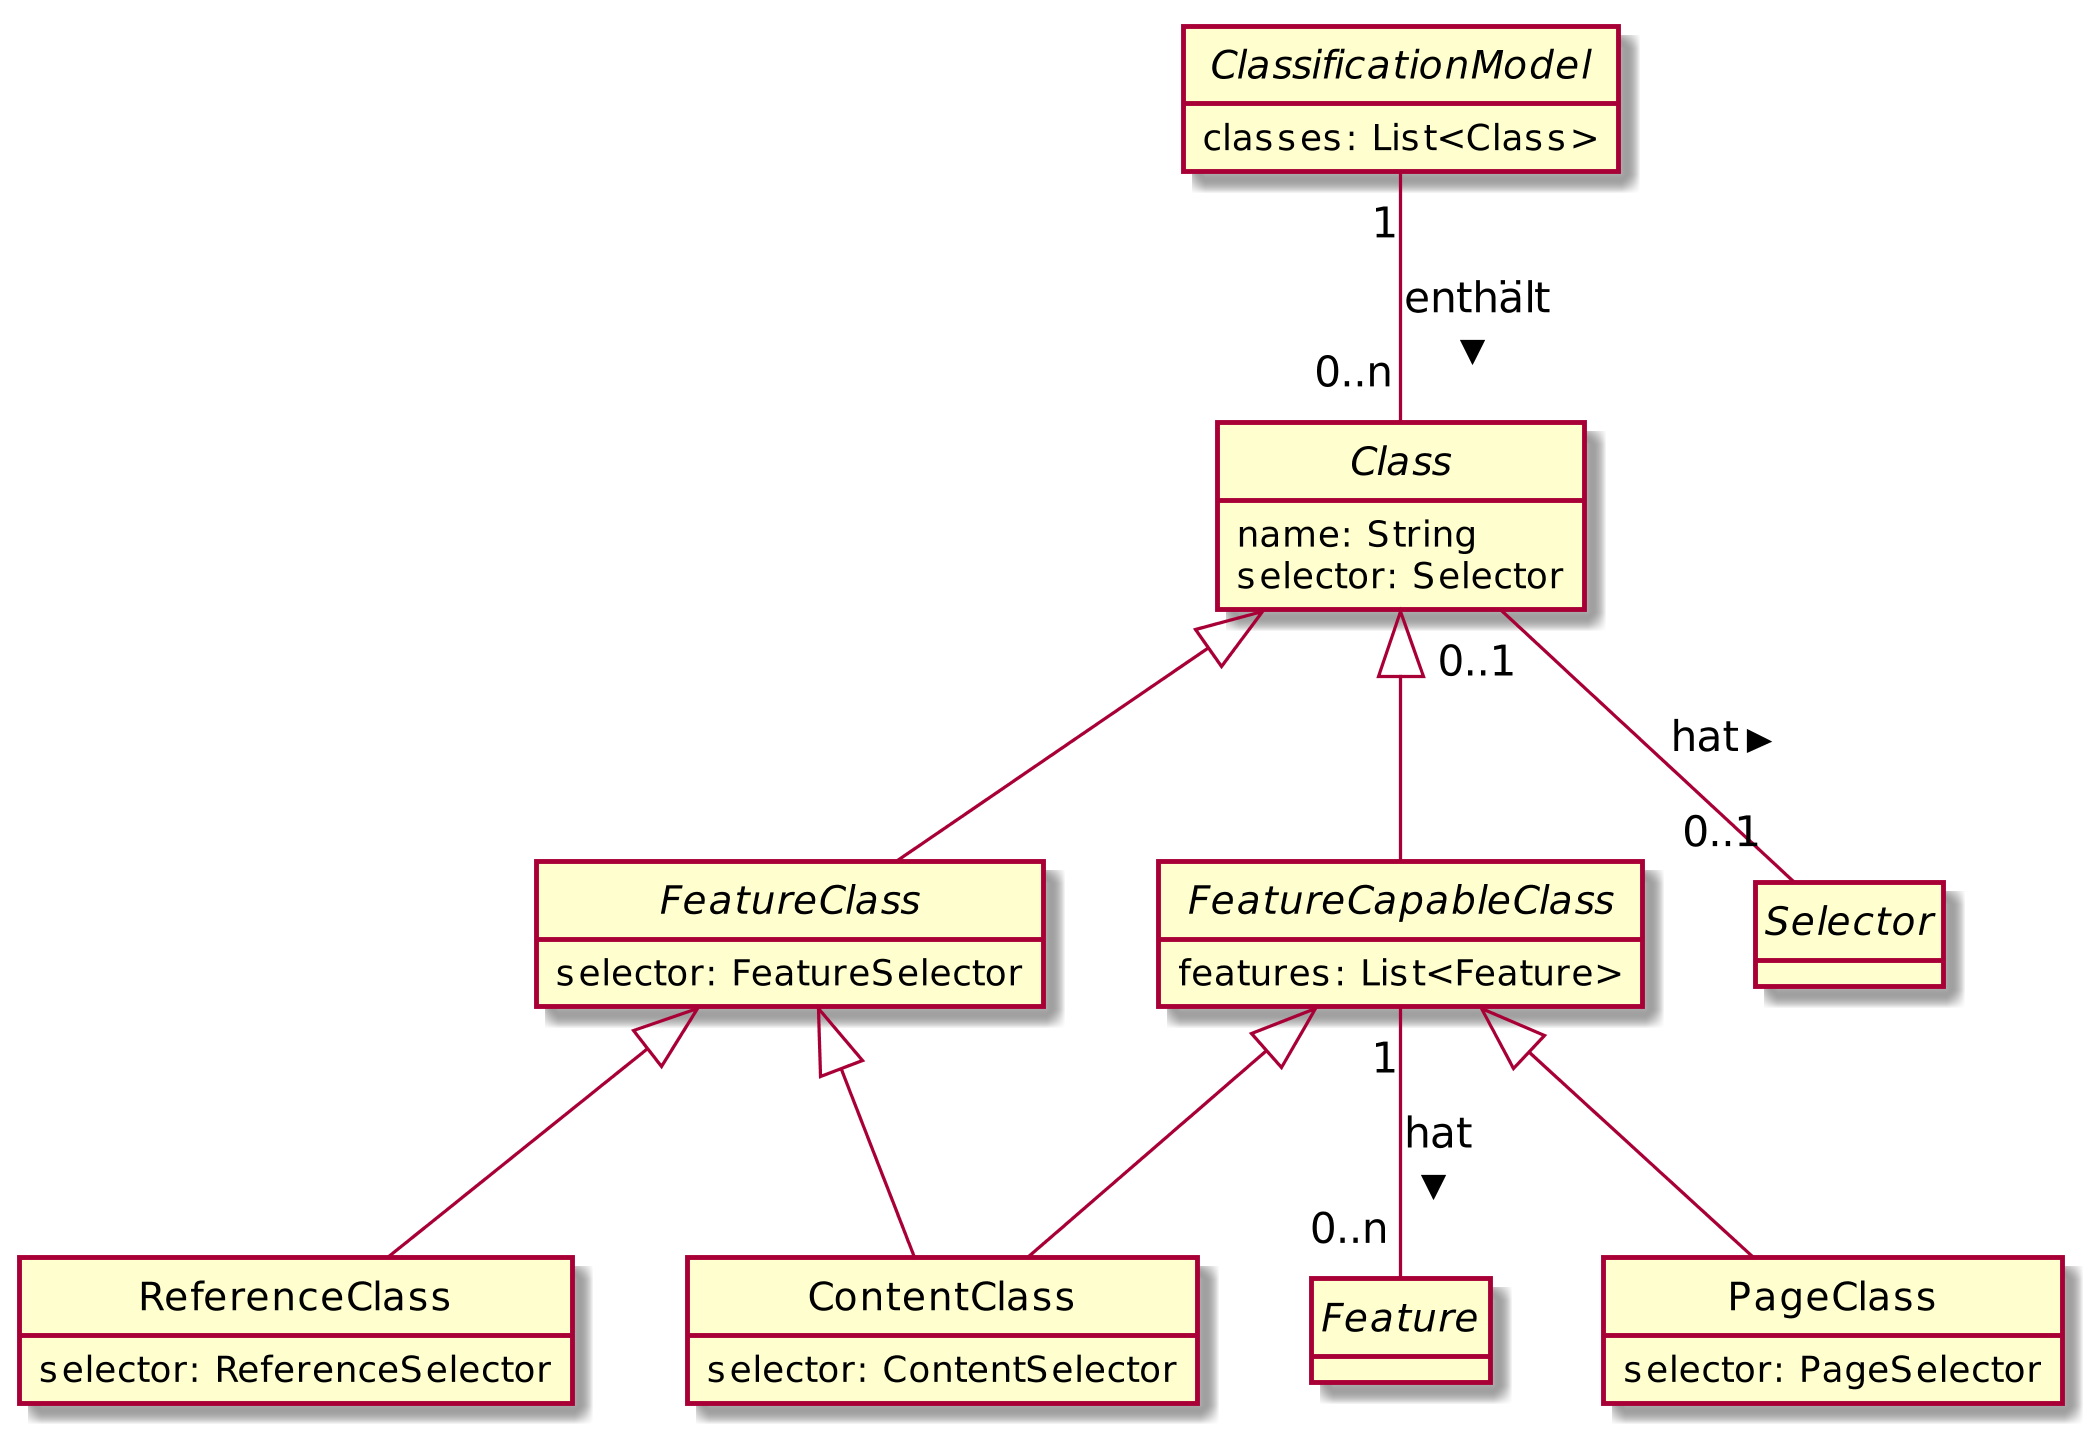
\includegraphics[width=\textwidth]{../resources/dsl/classes.png}
            \caption{Klassen in der DSL}
            \label{image:dslClasses}
        \end{figure}

        \begin{figure}
            \centering
            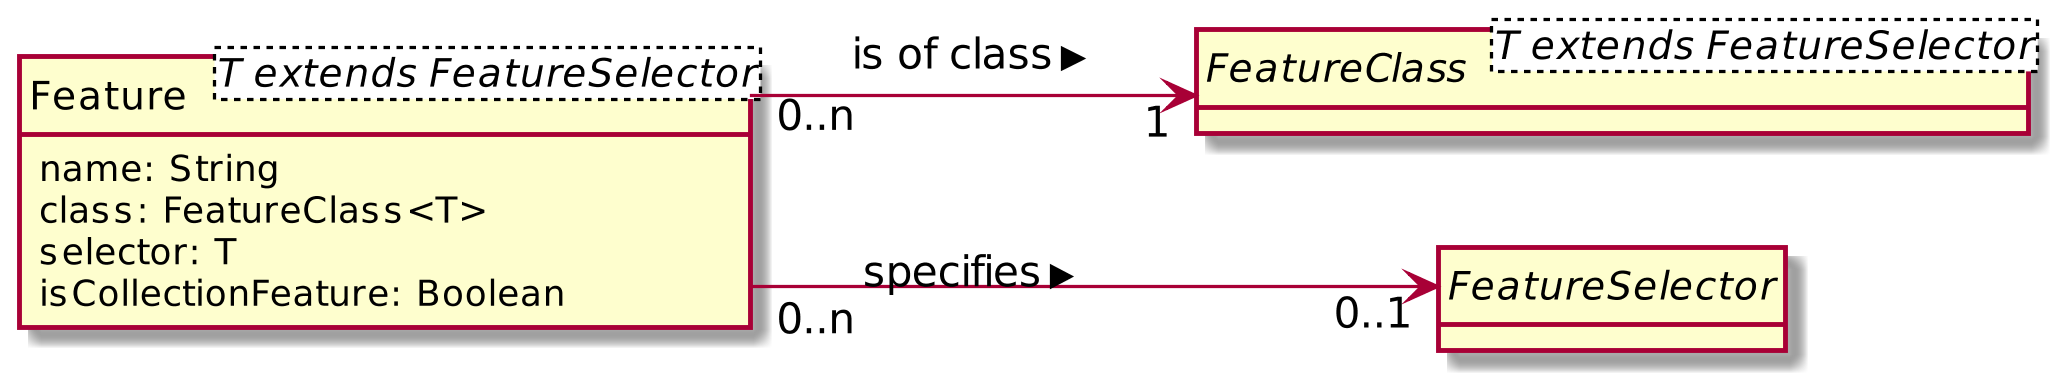
\includegraphics[width=\textwidth]{../resources/dsl/features.png}
            \caption{Features in der DSL}
            \label{image:dslFeatures}
        \end{figure}

        \begin{figure}
            \centering
            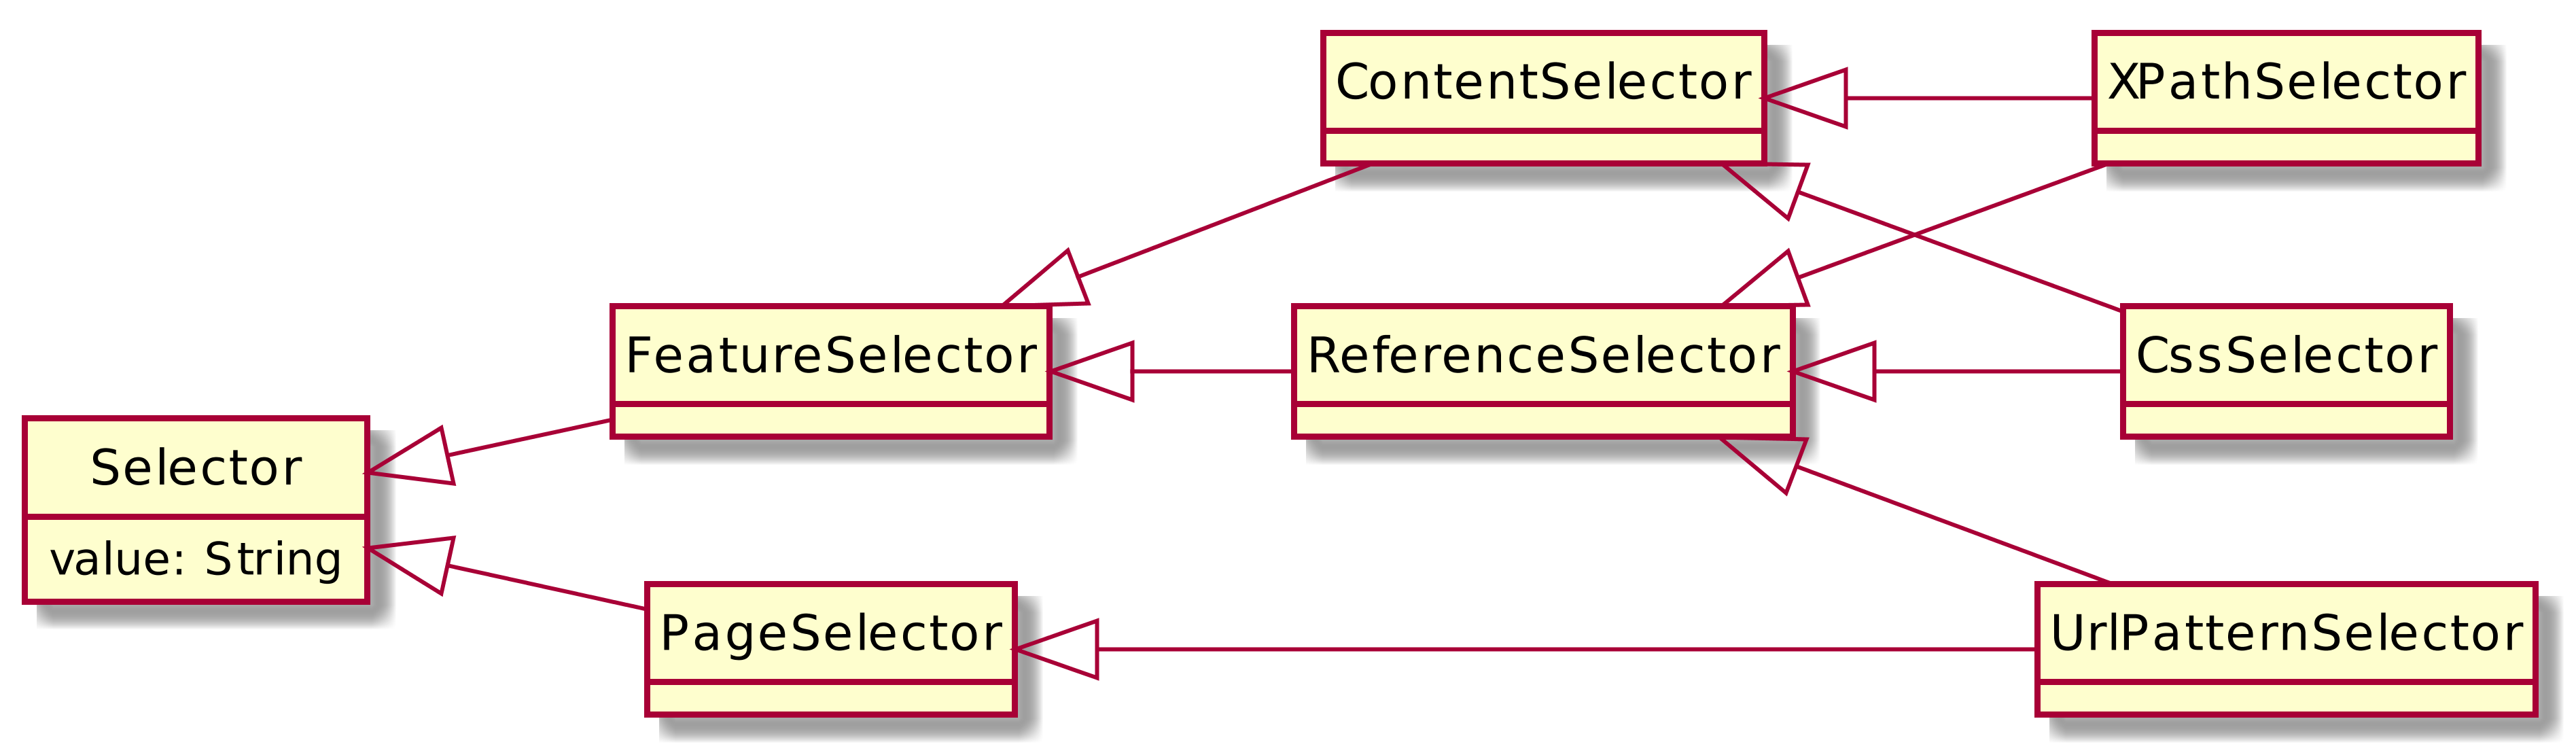
\includegraphics[width=\textwidth]{../resources/dsl/selectors.png}
            \caption{Selektoren in der DSL}
            \label{image:dslSelektoren}
        \end{figure}

    \subsection{Konkrete Syntax und deren Grammatik}
        \lstinputlisting[label=listing:dlsExample,caption=Beispielhafte Klassendeklaration]{../resources/dsl/example.wccd}    
        \lstinputlisting[label=listing:dlsGrammarClasses,caption=Klassen in der Grammatik der DSL]{../resources/dsl/grammar/classes.xtext}
        \lstinputlisting[label=listing:dlsGrammarSelectors,caption=Selektoren in der Grammatik der DSL]{../resources/dsl/grammar/selectors.xtext}
        \lstinputlisting[label=listing:dlsGrammarFeatures,caption=Features in der Grammatik der DSL]{../resources/dsl/grammar/features.xtext}

    \subsection{Transformation}
        \lstinputlisting[label=listing:dlsGenerationGlobal,caption=Erste Ebene]{../resources/dsl/generation/global.json}
        \lstinputlisting[label=listing:dlsGenerationPageClass,caption=Page Class]{../resources/dsl/generation/page-class.json}
        \lstinputlisting[label=listing:dlsGenerationFeature,caption=Feature]{../resources/dsl/generation/page-heading-feature.json}